\documentclass{beamer}					%printtaukseen [handout]
\usetheme{Frankfurt}
\usecolortheme{dove}

%\usepackage{pgfpages}							%printtaukseen
%\pgfpagesuselayout{2 on 1}[a4paper,border shrink=5mm]	%printtaukseen

\usepackage[T1]{fontenc}
\usepackage[utf8]{inputenc}
\usepackage{lmodern}
%\usepackage{natbib}							%for citations in Harvard style
\usepackage{xcolor}
\usepackage{amsmath}
\usepackage{mathtools}
\usepackage{amsfonts}
\usepackage{amssymb}
\usepackage{xfrac}
\usepackage[british]{babel}
\usepackage{cleveref}						%for multiple refs in one ref
\renewcommand*\familydefault{\ttdefault} %% Only if the base font of the document is to be typewriter style
\usepackage{courier}
\usepackage{booktabs}
\usepackage[backend=biber,citestyle=authoryear,bibstyle=authoryear]{biblatex}
\addbibresource{references.bib}
\usepackage{csquotes} % for proper quotation marks
\usepackage{textpos}

\DeclareMathOperator*{\E}{\mathbb{E}}				% Expectation symbol



%%%%% PATHS %%%%%

\graphicspath{{./plotit/}}
\DeclareGraphicsExtensions{.png,.pdf,.eps,.jpg}
%\addbibresource{refs.bib} %for citations

%%%% CUSTOMIZATION OF THE TEMPLATE %%%%%

\useinnertheme{rectangles} %rectangle bullets etc
\beamertemplatenavigationsymbolsempty	%no navigation bar
\setbeamercovered{transparent}		%future bullet points transparent 
\setbeamertemplate{frametitle}[default][colsep=-4bp,rounded=false,shadow=false] %no shadows
\definecolor{dark-gray}{gray}{0.80} %color for the navigation squares

%%%% FOOTLINE CUSTOMIZATION %%%%%

\setbeamercolor{section in head/foot}{fg=black, bg=white}
\makeatletter
\setbeamertemplate{footline}
{
	\leavevmode%
	\hbox{%
	\begin{beamercolorbox}[wd=.333333\paperwidth,ht=2.25ex,dp=1ex,center]{section in head/foot}%
		%\usebeamerfont{author in head/foot}\insertshortauthor~~
		%\beamer@ifempty{\insertshortinstitute}{}{(\insertshortinstitute)}
	\end{beamercolorbox}%
	\begin{beamercolorbox}[wd=.333333\paperwidth,ht=2.25ex,dp=1ex,center]{section in head/foot}%
 		%\usebeamerfont{title in head/foot}\insertshorttitle
	\end{beamercolorbox}%
	\begin{beamercolorbox}[wd=.333333\paperwidth,ht=2.25ex,dp=1ex,right]{section in head/foot}%
		%\usebeamerfont{date in head/foot}\insertshortdate{}\hspace*{2em}
		\insertframenumber{} / \inserttotalframenumber\hspace*{2ex} 
	\end{beamercolorbox}
    }%
	\vskip0pt%
}

%%%% HEADER CUSTOMIZATION %%%%%


\setbeamertemplate{mini frame}
{%
  \begin{pgfpicture}{0pt}{0pt}{.1cm}{.1cm}
    \pgfpathrectangle{\pgfpointorigin}{\pgfpoint{\the\beamer@boxsize}{\the\beamer@boxsize}}
    \pgfusepath{fill,stroke}
  \end{pgfpicture}%
}

\def\slideentry#1#2#3#4#5#6{%
  %section number, subsection number, slide number, first/last frame, page number, part number
  \ifnum#6=\c@part\ifnum#2>0\ifnum#3>0%
    \ifbeamer@compress%
      \advance\beamer@xpos by1\relax%
    \else%
      \beamer@xpos=#3\relax%
      \beamer@ypos=#2\relax%
    \fi%
  \hbox to 2pt{%
    \beamer@tempdim=-\beamer@vboxoffset%
    \advance\beamer@tempdim by-\beamer@boxsize%
    \multiply\beamer@tempdim by\beamer@ypos%
    \advance\beamer@tempdim by -.05cm%
    \raise\beamer@tempdim\hbox{%
      \beamer@tempdim=\beamer@boxsize%
      \multiply\beamer@tempdim by\beamer@xpos%
      \advance\beamer@tempdim by -\beamer@boxsize%
      \advance\beamer@tempdim by 1pt%
      \kern\beamer@tempdim
      \global\beamer@section@min@dim\beamer@tempdim
      \hbox{\beamer@link(#4){%
          \usebeamerfont{mini frame}%
          \ifnum\c@section>#1%
            \color{dark-gray}%
          \else%
            \ifnum\c@section=#1%
              \ifnum\c@subsection>#2%
                \color{dark-gray}%
              \else%
                \ifnum\c@subsection=#2%
                  \ifnum\c@subsectionslide>#3%
                    \color{dark-gray}%
                  \else%
                    \color{fg}%
                  \fi%
                \else%
                  \color{dark-gray}%
                \fi%
              \fi%
            \else%
              \color{dark-gray}%
            \fi%
          \fi%
          \usebeamertemplate{mini frame}%
        }}}\hskip-10cm plus 1fil%
  }\fi\fi%
  \else%
  \fakeslideentry{#1}{#2}{#3}{#4}{#5}{#6}%
  \fi\ignorespaces
  }
  
%%%% SOME BUG %%%%%

\def\pdftex@driver{pdftex.def}
\ifx\Gin@driver\pdftex@driver
  \def\pgfsys@color@unstacked#1{%
    \pdfliteral{\csname\string\color@#1\endcsname}%
  }
\fi

\makeatother



%%%%% INFORMATION ABOUT THE DOCUMENT %%%%%

\title[Thesis presentation]{Efficient Evidence Accumulation Clustering for large datasets / big data}

\author[Silva]{Diogo Alexandre Oliveira Silva \\ \tiny ALFAL / ENGEL}

\institute[AFA/IST]{
Academia da For\c{c}a A\'erea / Instituto Superior T\'ecnico \\
% \medskip
% %\textit{john@smith.com} % Your email address
% \vspace{2mm}
% \tiny \scalebox{1.2}{\textbf{J\'uri}}\\
% \vspace{2mm}
% \begin{tabular}{ll}
%  \tiny Presidente:						& \tiny Prof. Dr. Jo\~ao da Silva Sequeira\\ 
%  \tiny Orientador:						& \tiny Prof. Dr. Ana Lu\'sa Nobre Fred \\ 
%  \tiny Vogais:	 						& \tiny BGEN/ENGEL Luis Filipe Basto Dam\'asio\\
% 										& \tiny TCOR/ENGEL Ana Paula da Silva Jorge\\	
%  	 									& \tiny Prof. Dr. Pedro Filipe Zeferino Tom\'as\\
% \end{tabular}
}

\titlegraphic{
\includegraphics[scale=0.06]{afa}\hfill%\hspace*{4.75cm}~%
   
\includegraphics[scale=0.14]{IST_A_CMYK_POS}
}

\date{November, 2015}

					  
%%%%% ACTUAL DOCUMENT PAGES %%%%%					  

\begin{document}


\begin{frame}[plain]

%Instirutions symbols
%\begin{flushleft}
%
\includegraphics[bb=4cm 11cm 0cm 0cm,scale=0.14]{IST_A_CMYK_POS}
%
\includegraphics[bb=-186cm 15cm 0cm 0cm,scale=0.06]{afa}

% 
\includegraphics[bb=4cm 13cm 0cm 0cm,scale=0.14]{IST_A_CMYK_POS}
% 
\includegraphics[bb=-180cm 16cm 0cm 0cm,scale=0.05]{afa}
%\end{flushleft}

% \begin{textblock}{20}(0,0)
%       
\includegraphics[scale=0.14]{IST_A_CMYK_POS}
% \end{textblock}

% \begin{picture}(0,0)
% \put(100,100){\hbox{
\includegraphics[scale=0.14]{IST_A_CMYK_POS}}}
% \end{picture} 

% \begin{figure}
% \centering
% \begin{minipage}{.5\textwidth}
%   \centering
%   
\includegraphics[scale=0.14]{IST_A_CMYK_POS}
% \end{minipage}%
% \hfill
% \begin{minipage}{.5\textwidth}
%   \centering
%   
\includegraphics[scale=0.06]{afa}
% \end{minipage}
% \end{figure}

\titlepage

\end{frame}

%--------------------------------------------%
%    OVERVIEW 
%--------------------------------------------%

\begin{frame}
\frametitle{Contents} % Table of contents slide, comment this block out to remove it
\footnotesize \tableofcontents % Throughout your presentation, if you choose to use \section{} and \subsection{} commands, these will automatically be printed on this slide as an overview of your presentation
\end{frame}

          


\chapter{Introduction}
\label{chapter:introduction}

%TODO (extra introduction)
% problems under Big Data paradihm
% typical challenges with Big Data
% why EAC?
% combination of both

\section{Challenges and Motivation}

% Estrutura mais clara:
% Motivacao: analise atomatica de dados numa perspectiva de
% analise exploratoria; exemplos; novos desafios face a grande
% quantidade de dados; tecnicas de clustering como as tecnicas
% formais de abordar estes problemas; dificuldades tradicionais
% que levaram ao state-of-art dos metodos de ensemble.
% Dificuldades adicionais asociados ao Big Data; face a isto a
% tese propoe abordar este problema ....
 
% Se quizeres, formulacao mais detalhada do problema com um
% exemplo mais motivador com dados reais: clustering, EAC, ...



% Motivacao: analise atomatica de dados numa perspectiva de
% analise exploratoria;
Advances in technology allow for the collection and storage of unprecedented amount and variety of data, a concept commonly designated by \emph{Big Data}.
Most of this data is stored electronically and there is an interest in automated analysis for generation of knowledge and new insights.
%examples of applications; jet engine example is nice for Air Force: taken from http://wikibon.org/wiki/v/Big_Data_in_the_Aviation_Industry; related Carnegie Mellon: http://bigdatasymposium.dsigroup.org/wp-content/uploads/2011/12/Dubrawski-DSI-Big-Data-Symposium-January-29-2013.pdf
The applications of such analysis are abundant and across many fields, ranging from recommender systems and customer segmentation in business, to predicting when a jet engine is likely to fail using sensor data, or even the study of gene expression in biomedics, to namy a few.

% examples of analisis tools
A growing body of statistical methods aiming to model, structure and/or classify data already exist, e.g. linear regression, principal component analysis, cluster analysis, support vector machines, neural networks.
% tecnicas de clustering como as tecnicas formais de abordar estes problemas
Cluster analysis is an interesting tool because it typically does not make assumptions on the structure of the data.
Since, often, the structure of the data is unknown, clustering techniques become particularly interesting for transforming this data into knowledge and discovering its underlying structure and patterns.
%Clustering is a ill defined problem, one of the reasons why there are hundreds of algorithms. 
Clustering is a hard problem and a vast body of work on these algorithms exist.
Yet, typically, no single algorithm is able to respond to the specificities of all data.
Different methods are suited to datasets of different characteristics and, often, the challenge of the researcher is to find the right algorithm for the task. %TODO get ref for this

% dificuldades tradicionais que levaram ao state-of-art dos metodos de ensemble.
Currently, there are state of the art algorithms that are more robust than "traditional" algorithms by having a wider applicability or being less dependent on input parameters, e.g. algorithms that do not take any parameters for performing an analysis.
One such algorithm is Evidence Accumulation Clustering (EAC), belonging to the wider class of ensemble methods.
EAC is a state-of-the art clustering algorithm that addresses the robustness challenge.
% novos desafios face a grande quantidade de dados; % Dificuldades adicionais asociados ao Big Data
However, the current reality of capturing massive amounts of data rises new challenges.
Two important challenges are efficiency and scalability, which translate on how fast the algorithms are and how well they scale when the input data multiplies in size, dimensionality and variety.
The algorithms themselves are no longer the only focus of research.
Much effort is being put into the scalability and performance of algorithms, which usually translates in addressing their computational complexity with parallelized computation and distributed memory being some of the proposed solutions.
Cluster analysis with EAC should be fast and able to scale to larger datasets as well as robust, so as to address the reality of big data.

%TODO review paragraph; it is a collection of phrases right now
% This sprouted the rise of new uses of existing computing architectures (e.g. Graphic Processing Units) and development of new programming models (e.g. Hadoop, shared and distributed memory).
% Each of these has its own specificities and the researcher must have an in-depth knowledge of the architectures and models used to frame the problems and obtain results.

% face a isto a tese propoe abordar este problema
This dissertation is concerned with pushing the current limits of the EAC to large datasets by addressing the problems of scalability and efficiency without compromising robustness, using technology available in a desktop workstation.
Processing of huge amounts of data has been out of the range of capability of the traditional desktop workstation.
This sprouted the rise of new uses of existing computing architectures (e.g. Graphic Processing Units) and development of new programming models (e.g. Hadoop, shared and distributed memory).
The problem at hand is, then, to  optimize the algorithm regarding both speed and memory usage.
This, of course, comes with challenges.
How can one keep the original accuracy while significantly increase efficiency?
Is there an exploitable trade-off between the three main characteristics: speed, memory and accuracy?
These are guiding questions that this dissertation addresses.


\section{Goals}

This dissertation aims to research and extend the state of the art of ensemble clustering, in what concerns the EAC method and its application to large datasets, while also assessing algorithmic solutions and parallelization techniques.
The goal is to understand EAC's suitability for large datasets and find ways to respond to the stated challenges, in terms of speed and memory.
The main objectives for this work are:

\begin{itemize}

\item Study the integration of quantum inspired methods in EAC.

\item Study the integration of the General Purpose computing in a Graphics Processing Unit (GPGPU) paradigm in EAC.

\item Devise strategies to reduce computation and memory complexities of EAC.

\item Application of Evidence Accumulation Clustering to Big Data.

\item Validation of Big Data EAC on real data.% (ECG for emotional state discovery and/or discovery of natural groups, or other datasets)
\end{itemize}

\section{Contributions}
The main contributions are the adaptation of the three distinct stages of the EAC framework to larger datasets.
In particular, an efficient parallel version for Graphics Processing Units (GPU) of the K-Means clustering algorithm is implemented for the first stage of EAC.
Still in this stage, two clustering algorithms in the young field of Quantum Clustering were reviewed, tested and evaluated having EAC in mind. % QK-Means and Horn
Different methods for the second stage were tested, using complete matrices and sparse matrices.% and a k-Nearest Neighbors scheme.
Worthy of mention is a novel and specialized method for building a sparse matrix in the second stage. % EAC CSR
%A post-processing operation on the second stage product was briefly studied. % the threshold cut
A GPU parallel version of a MST (Minimum Spanning Tree) solver algorithm was reviewed and tested for the last stage, a co-product of which was an algorithm to find the connected components of a MST.
A hard disk solution was implemented for dealing with large datasets whose space complexity in the final stage exceeded the available memory.


% Explain briefly the work done

% The scope of the thesis is Big Data and Cluster Ensembles.
% A main requirement in this context is to have fast clustering techniques.
% This may be accomplished in two ways: algorithmically or with parallelization techniques.
% The former deals with finding faster solutions while the latter takes existing solutions and optimizes them with execution speed in mind.

% The initial research was under the algorithmic path.
% More specifically, exploring quantum inspired clustering algorithms.
% The findings of this exploration revealed this algorithms to be a poor match for integration in EAC and turned the focus of the research to parallelization techniques.
% Two main paradigms of parallelization were found appropriate: GPGPU and distributed (among a cluster of workstations).
% While the first is a readily available resource in common machines, the second is able to address problems dealing with larger datasets.

\section{Outline}

Chapter \ref{chapter:clustering} provides an introduction to clustering nomenclature and concepts, as well as some "traditional" clustering algorithms.
Chapter \ref{chapter:stateofart} starts by reviewing the Evidence Accumulation Clustering algorithm in detail.
It goes on to review possible approaches to the problem of scaling EAC.
Based on an algorithmic approach, a review of the young field of quantum clustering is presented, with a more in-depth emphasis on two algorithms.
With a parallelization approach in mind, a programming model for the GPU (CUDA) is reviewed, followed by some parallelized versions of relevant algorithms to the problem of this dissertation.
The following chapter, \ref{chapter:methodology}, presents the approach that was actually taken to scale EAC.
It presents the steps taken on each part of the algorithm, the underlying difficulties and what was done to address them.
It also includes the reference of approaches that were developed but were not deemed suited to integrate the EAC toolchain.
In the results chapter, \ref{chapter:results}, the results of the different approaches of optimizing the EAC method are presented.
Chapter \ref{chapter:discussion} presents an interpretation and critical discussion of those results.
Finally, chapter \ref{chapter:conclusions} concludes the dissertation.
It also offers recommendations for future work.
%--------------------------------------------%
%--------------------------------------------%
%    PROPOSED SOLUTION 
%--------------------------------------------%
%--------------------------------------------%

\section{Proposed solution}

\subsection{Overview}

% FRAME: OVERVIEW OF PROPOSED SOLUTION
\begin{frame}{Proposed solution: overview}
\begin{figure}[hbt!]
  \centering
  \includegraphics[width=0.8\columnwidth]{{{diagram_proposed_solutions}}}
  %\caption{[1] A. N. L. Fred and A. K. Jain, “Combining multiple clusterings using evidence accumulation,” IEEE Transactions on Pattern Analysis and Machine Intelligence, vol. 27}
  \label{fig:eac kmin evo}
\end{figure}

\end{frame}

\begin{frame}{Proposed solution: final}
\begin{figure}[hbt!]
  \centering
  \includegraphics[width=1.0\columnwidth]{{{diagram_proposed_solutions_BAD}}}
  %\caption{[1] A. N. L. Fred and A. K. Jain, “Combining multiple clusterings using evidence accumulation,” IEEE Transactions on Pattern Analysis and Machine Intelligence, vol. 27}
  \label{fig:eac kmin evo}
\end{figure}

\end{frame}

%--------------------------------------------%
%    PRODUCTION PHASE
%--------------------------------------------%
\subsection{Production}

\begin{frame}{Optimizing production of ensemble}

\begin{itemize}

\item K-Means is simple and has been used with EAC before with success.

\item K-Means:

  \begin{itemize}
  \item \textbf{labelling}: find the closest centroid to each data pattern
  % $$
  % l_i = arg \: \min_k \;d(x_i, c_k)
  % $$
  \item \textbf{update}: new centroids are the mean of the assigned patterns
  % $$
  % c_k = \sum_{i : l_i = k} x_i
  % $$

  \end{itemize}

\item Number of clusters from interval [$K_{min},K_{max}$]

\item Optimization through parallelization in GPU.

\end{itemize}

\end{frame}



\begin{frame}{GPGPU K-Means}

\begin{itemize}

\item CUDA GPGPU

  \begin{itemize}
  \item Hundreds of processors

  \item \emph{Single instruction multiple thread} approach

  \item Shared memory between threads

  \end{itemize}
\end{itemize}

\end{frame}



\begin{frame}{GPU K-Means}

\begin{itemize}

% \item CUDA GPGPU
\item GPU

  \begin{itemize}
  \item Hundreds of processors

  \item \emph{Single instruction multiple thread} approach

  \item Shared memory between threads

  \end{itemize}

\item Parallel K-Means

  \begin{enumerate}

  \item Host sends data and centroids to GPU

  \item GPU threads compute the closest centroid to data patterns.

  \item The label and distance are stored and transfered to host.

  \item Host computes new centroids and sends them back to host.

  \item Repeat steps 2-4 until stopping criteria is met.

  \end{enumerate}

\end{itemize}

\end{frame}



        
%--------------------------------------------%
%    COMBINATION PHASE
%--------------------------------------------%
\subsection{Combination}

\begin{frame}{Optimizing combination}

\begin{itemize}

\item Biggest challenge: $O(n^2)$ memory complexity
  \begin{itemize}
  \item $200\:000$ dataset $\longrightarrow$ $149$ GB
  \item $1\:000\:000$ dataset $\longrightarrow$ $3725$ GB
  \end{itemize}

\item Co-association matrix is:
  \begin{itemize}
  \item symmetric ($49.5\%$ reduction)
  \item sparse (association density as low as $1\%$)
  \end{itemize}

\item \textbf{exploiting sparsity}

% \item Two approaches:
%   \begin{itemize}
%   \item using prototypes
%   \item \textbf{exploiting sparsity}
%   \end{itemize}

\end{itemize}

\begin{center}
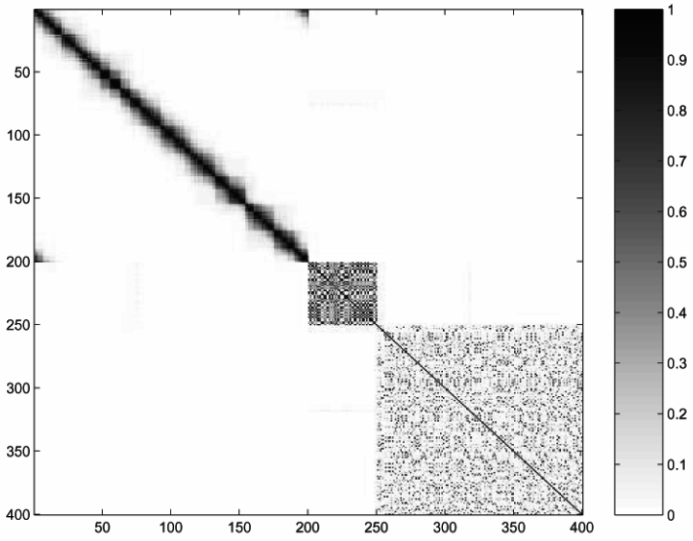
\includegraphics[width=0.3\textwidth]{EAC_plots/coassocEAC}
\end{center}

\end{frame}



\begin{frame}{Optimizing combination}

\begin{itemize}

%\item Sparse formats: LIL, DOK, COO, CSR, CSC

\item Library solutions are either very slow or occupy too much memory

\item Lack of literature on fast building

\item Compromise between speed and memory: \\
\centering
\Large{\textbf{EAC CSR}}

  % \begin{itemize}
  % \item \Large{\textbf{EAC CSR}}
  % \end{itemize}

\end{itemize}

\end{frame}


% plot for coming up with assumption for number of associations
% \begin{frame}{Optimizing combination}
% \begin{center}
%   \includegraphics[width=0.8\columnwidth]{{{max_assoc_bgs}}}
% \end{center}
% \end{frame}


\begin{frame}{Optimizing combination}
\begin{center}
  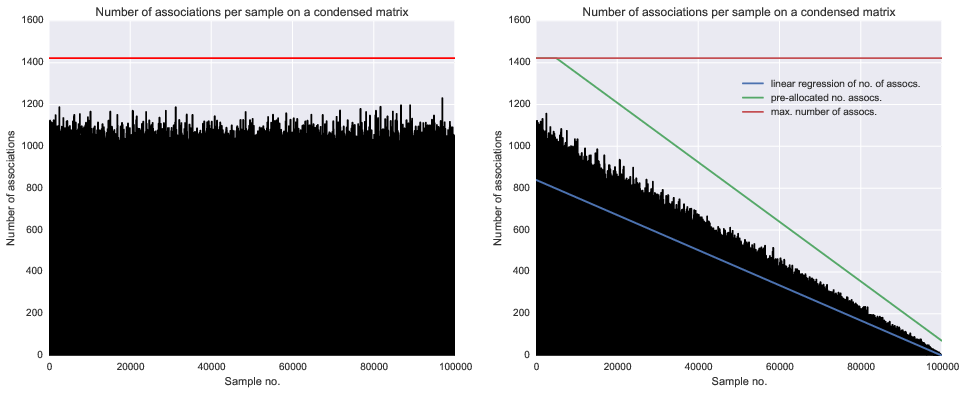
\includegraphics[width=0.8\columnwidth]{eac_csr_cond_full_degree_100k.png}
\end{center}
\end{frame}


%--------------------------------------------%
%    RECOVERY PHASE
%--------------------------------------------%
\subsection{Recovery}

\begin{frame}{Optimizing final clustering}

\begin{itemize}

\item Single-Link (SL) has been used before with success

\item SL is a hierarchical agglomerative algorithm

\item SL works on a pair-wise proximity matrix between all patterns

\item SL is equivalent to a Minimum Spanning Tree (MST)

\item Disk based MST variant to address very large co-association matrices

\end{itemize}

% used MST based Single-Link to process only real associations.
% Used out-of-core sorting algorithm from PyTables for sorting the associations.
\end{frame}
%!TEX root = thesis.tex


\section{Results}
\subsection{Quantum K-Means}


The algorithm implemented and tested is a variant of the one described in ~\cite{Casper}. The genetic operations of cross-over and mutation are both part of the genetic algorithms toolbox, but were not implemented due to the suggestion from ~\cite{Wiebe2014}. This decision was based on the findings of ~\cite{Liu2010}, stating that the use of the angle-distance rotation method in the quantum rotation operation produces enough variability, with a careful choice of the rotation angle.

\subsubsection{Testing and Results}
The testing was aimed at benchmarking both accuracy and speed. The input used was synthetic data, namely, Gaussian mixtures with variable cardinality and dimensionality. The algorithm was implemented in Python 2.7 and the tests were executed in a machine with an Intel i5 processor, 2GB RAM and running Ubuntu 14.04.

(copy of report)

Regarding the Quantum K-Means (QK-Means), the tests were performed using 10 oracles, a qubit string length of 8 and 100 generations per round. The \textbf{classical} K-Means was executed using the \textbf{k-means++} centroid initialization method, since QK-Means also has some computational cost in the beginning of the algorithm.. Since QK-Means executes a classical K-Means for each oracle each generation, the number of initializations for K-Means was $num.oracles \times num.generations \times factor$, where $factor$ is an adjustable multiplier. Each test had 20 rounds t allow for statistical analysis of the results.

All tests were done with 6 clusters (natural number of clusters). Two tests were done with the two dimensional dataset: one with a $factor=1.10$ (increase initializations by $10\%$) and another with $factor=1$. These tests will be called T1 and T2, respectively. The test done with the six dimensional dataset (T3) used $factor=1.10$.

Timing results

% table in csv format available in resource directory -->

\begin{table}[h]
\caption{Timing results for the different algorithms in the different tests. Fitness time refers to the time that took to compute the DB index of each solution of classical K-Means. All time values are the average over 20 rounds and are displayed in seconds.}
\begin{tabular}{|l|l|l|l|l|l|}
\hline
\textbf{Dataset}               & \textbf{Algorithm} & \textbf{Mean} & \textbf{Variance} & \textbf{Best} & \textbf{Worst} \\ \hline
\textbf{T1}                    & QK-Means           & 62.02642975   & 0.077065212       & 61.620424     & 62.579969      \\ \cline{2-6} 
\textbf{bi36}                  & K-Means            & 6.4774672     & 0.002501651       & 6.352554      & 6.585451       \\ \cline{2-6} 
\textbf{}                      & K-Means + fitness  & 70.2238286    & 0.022223755       & 69.889105     & 70.548572      \\ \cline{2-6} 
\textbf{}                      & fitness            & 63.7463614    & 0.019722105       & 63.536551     & 63.963121      \\ \hline
\textbf{T2}                    & QK-Means           & 64.22347165   & 0.056559152       & 63.807367     & 64.807373      \\ \cline{2-6} 
\textbf{bi36 noFactor} & K-Means            & 5.71167475    & 0.004903253       & 5.581391      & 5.877091       \\ \cline{2-6} 
\textbf{}                      & K-Means + fitness  & 62.7021533    & 0.066919692       & 63.417207     & 62.180021      \\ \cline{2-6} 
\textbf{}                      & fitness            & 56.99047855   & 0.062016439       & 56.59863      & 57.540116      \\ \hline
\textbf{T3}                    & QK-Means           & 74.4917966    & 0.067688312       & 74.12105      & 74.976446      \\ \cline{2-6} 
\textbf{sex36}                 & K-Means            & 8.291648      & 0.007015777       & 8.160859      & 8.426203       \\ \cline{2-6} 
                               & K-Means + fitness  & 72.36315915   & 0.05727269        & 71.856457     & 73.031841      \\ \cline{2-6} 
                               & fitness            & 64.07151115   & 0.050256913       & 63.695598     & 64.605638      \\ \hline
\end{tabular}
\end{table}

The mean computation time of classical K-Means is an order of magnitude lower than that of QK-Means. However, in classical K-Means the solution typically chosen is the one with lowest sum of squared euclidean distances of points to their attributed centroid. To make a fair comparison between the two algorithms, the Davies-Bouldin index of all classical K-Means solutions was computed and used as the criteria to choose the best solution. When this is done, we can see that the total time of classical K-Means is actually higher that that of QK-Means in T1 and T3, but this is only due to the 1.10 multiplier on the number of initializations. In T2, possibly the fairest comparison, the computation times become very similar with only a 2\% difference between the two algorithms.

Accuracy

Comparing K-Means and QK-Means

% table in csv format available in resource directory -->

\begin{table}[h]
\caption{All values displayed are the average over 20 rounds, except for the Overall best which shows the best result in any round. The values represent the Davies-Bouldin fitness index (low is better).}
\begin{tabular}{|l|l|l|l|l|l|l|}
\hline
\textbf{Dataset} & \textbf{Algorithm} & \textbf{Best} & \textbf{Worst} & \textbf{Mean} & \textbf{Variance} & \textbf{Overall best} \\ \hline
\textbf{T1}      & QK-Means           & 15.42531927   & 32.29577426    & 19.94704511   & 21.23544567       & 15.42531927           \\ \cline{2-7} 
\textbf{}        & K-Means            & 15.42531927   & 25.44913817    & 16.25013365   & 1.216919278       & 15.42531927           \\ \hline
\textbf{T3}      & QK-Means           & 22.72836641   & 65.19984617    & 36.10699242   & 78.14043743       & 22.71934191           \\ \cline{2-7} 
\textbf{}        & K-Means            & 22.71934191   & 46.72231967    & 26.18440481   & 22.96730826       & 22.71934191           \\ \hline
\end{tabular}
\end{table}

The most relevant result in the table above is the mean of the best index. The value is the average over all rounds of the best solution in each round and it provides insight on the average performance of the algorithm. The results suggest that both algorithms perform equally well. The best overall result of each algorithm in all rounds is exactly the same. In T3, the mean performance of classical K-Means is marginally better.

I speculate that if classical K-Means was using only the sum of euclidean distances and not the DB index, the average performance would be worse. As it stands, choosing to use DB index with classical K-Means possibly represents a tradeoff between speed and accuracy.

QK-Means details

Here we’ll analyse a bit what’s happening within each QK-Means execution. One would expect for the population’s fitness variance to decrease over the generations, as the probabilities for previous known solutions increase and are therefore more likely to reappear. The convergence of the population mean would also be expected to decrease for the same reason. However, experimental (Fig. \ref{fig:db_index_mean_t2} and \ref{fig:db_index_var_t2}) results don’t suggest any of these expectations (the results of T1 and T3 suggest the same). This may be due to low number of generations or simply because the random generation of initial centroids isn’t influenced enough by the qubit probabilities.


\begin{figure}[hbtp]
\centering
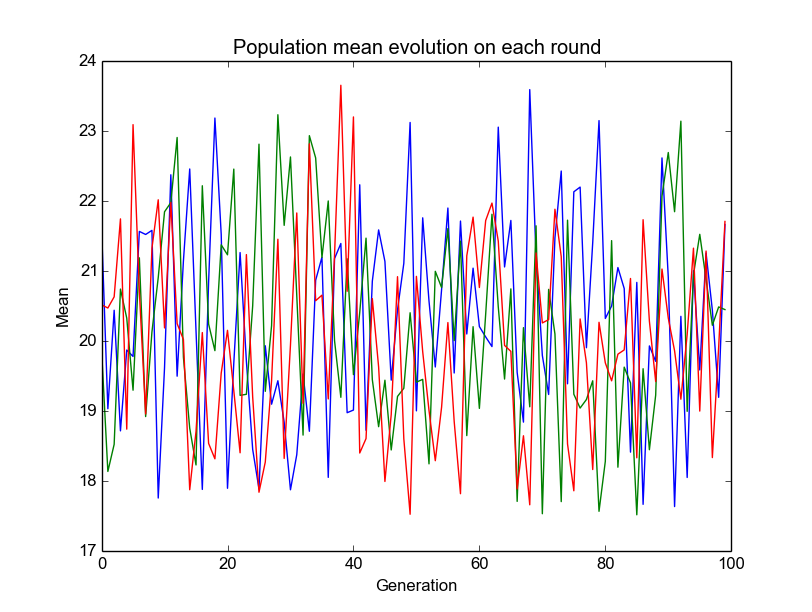
\includegraphics[scale=0.5]{QK_Means/img/bi_nofactor_mean.png}
\caption{DB index mean of the population in T2. Only 4 rounds represented.}
\label{fig:db_index_mean_t2}
\end{figure}

\begin{figure}[hbtp]
\centering
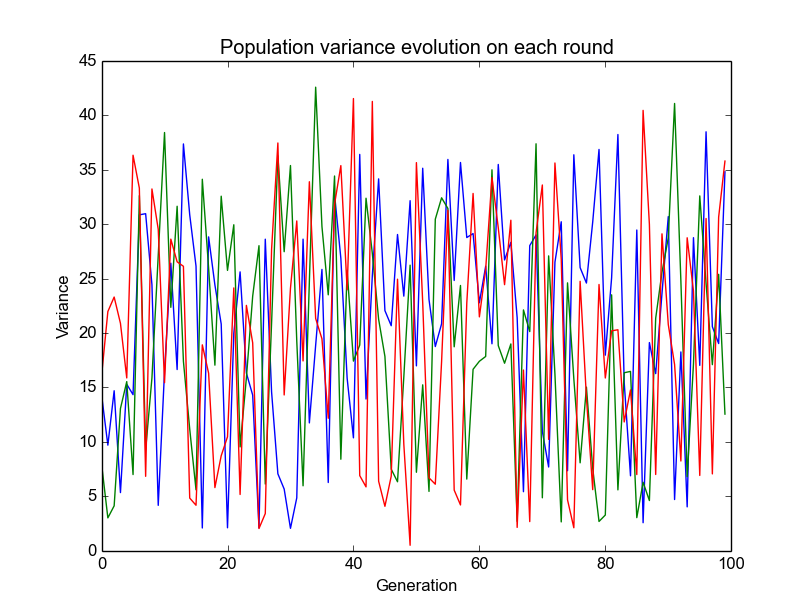
\includegraphics[scale=0.5]{QK_Means/img/bi_nofactor_var.png}
\caption{DB index variance of the population in T2. Only 4 rounds represented.}
\label{fig:db_index_var_t2}
\end{figure}


Analysing the evolution of the DB index of the best solution over the generations (Fig. \ref{fig:qk_db_index_best_evo_t2} and \ref{fig:qk_db_index_best_evo_t3}) gives some insight on the rate of convergence. In both tests it is clear that the best solution is often reached in a quarter of the total generations. More detail can be seen in the Table \ref{tab:db_index_t1_t3}.

\begin{figure}[hbtp]
\centering
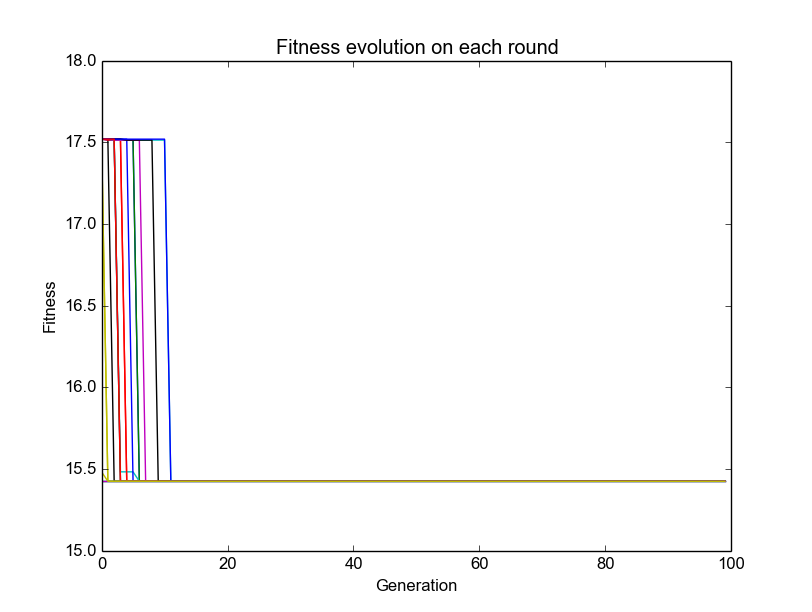
\includegraphics[scale=0.5]{QK_Means/img/bi_nofactor_evo.png}
\caption{DB index of best solution in T2.}
\label{fig:qk_db_index_best_evo_t2}
\end{figure}


\begin{figure}[hbtp]
\centering
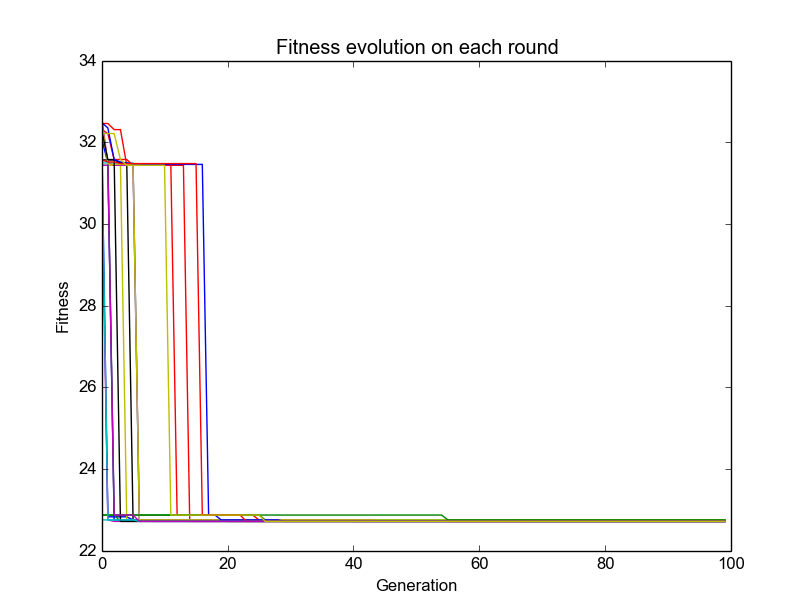
\includegraphics[scale=0.5]{QK_Means/img/sex_evo.png}
\caption{DB index of best solution in T3.}
\label{fig:qk_db_index_best_evo_t3}
\end{figure}

% table in csv format available in resource directory -->

\begin{table}[h]
\caption{The values represent generations.}
\begin{tabular}{|l|l|l|l|l|}
\hline
\textbf{Test} & \textbf{Mean} & \textbf{Variance} & \textbf{Best} & \textbf{Worst} \\ \hline
\textbf{T1}   & 17.25         & 70.2875           & 3             & 33             \\ \hline
\textbf{T3}   & 28.05         & 568.6475          & 2             & 90             \\ \hline
\end{tabular}
\label{tab:db_index_t1_t3}
\end{table}

\subsubsection{Discussion}

Results show that most computational cost (90\% on T1) lies on the evaluation of the solutions obtained from each oracle. This is a costly but necessary step in this algorithm. Moreover, and even though EAC doesn't require its input partitions to be accurate, the quality of the solutions, measured with the Davies-Bouldin index, from QK-Means doesn't differ from that of K-Means. This two facts make the use of this algorithm in EAC prohibitive, as no benefits in compuational time are gained.

It should be noted that the target application of the tests presented differs from that of the original authors and although no accuracy gains were observed in these results, the results might differ on different applications.

\subsection{Horn and Gottlieb's algorithm}


\subsubsection{Testing and Results}


%TODO
%Put in accuracy results for crab,iris and gaussian mixtures  
%Put in timing results


The accuracy of this algorithm was tested with real world datasets, namely, the crab and iris datasets available at the UCI Machine Learning Repository.

%TODO add ref for repository -->

\subsubsection{Iris data}
\label{sec:horn_iris}
The iris dataset ([available at the UCI ML repository](http://archive.ics.uci.edu/ml/datasets/Iris)) has 3 classes each with 50 data points. There are 4 features. The data is preprocessed using Principal Component Analysis (PCA). The natural clustering can be observed in Fig. \ref{fig:iris_natural}. 

% #TODO saved image from ipython -->

\begin{figure}[hbtp]
\centering
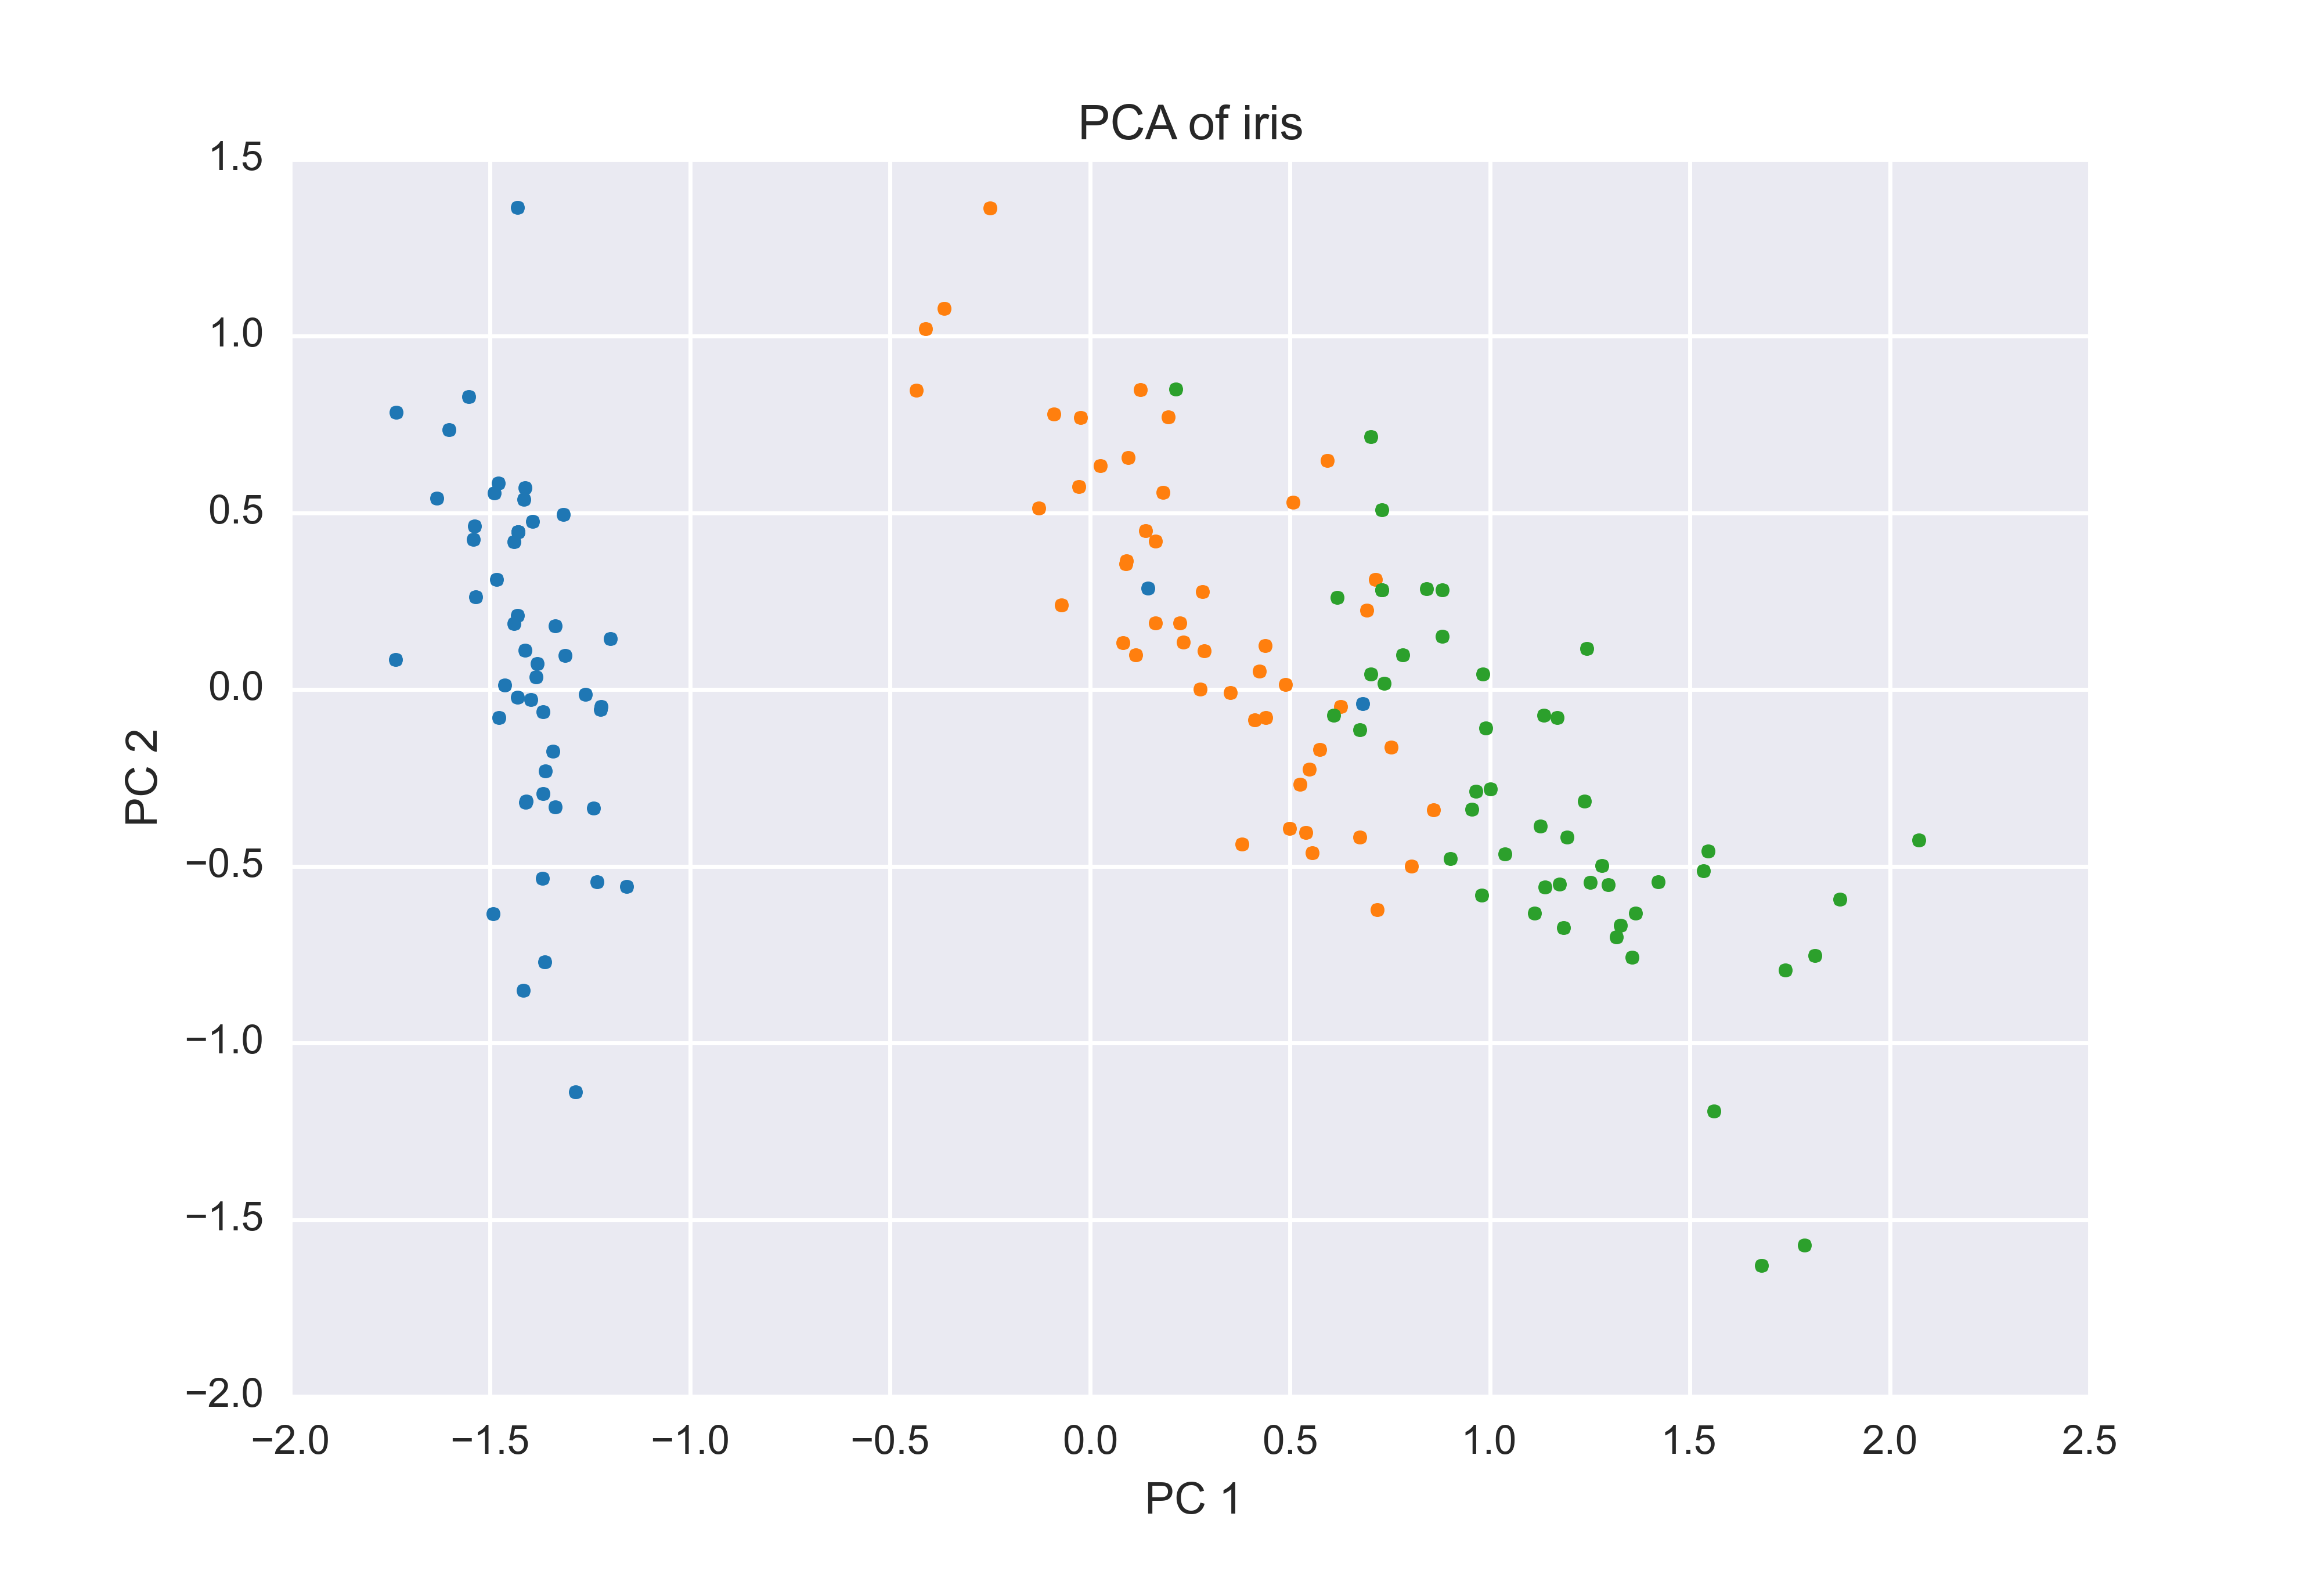
\includegraphics[scale=0.5]{Horn/img/iris_natural.png}
\caption{Plot of the two first principal components (PC).}
\label{fig:iris_natural}

\end{figure}

I chose $\sigma=\frac{1}{4}$ to reproduce the experiments in [3]. Only the first two PC are used here, which account for $95.8\%$ of the energy. The clustering results can be seen in Fig. \ref{fig:iris_2pc_cluster} and have an accuracy of 86\% computed with consistency index.


\begin{figure}[hbtp]
\centering
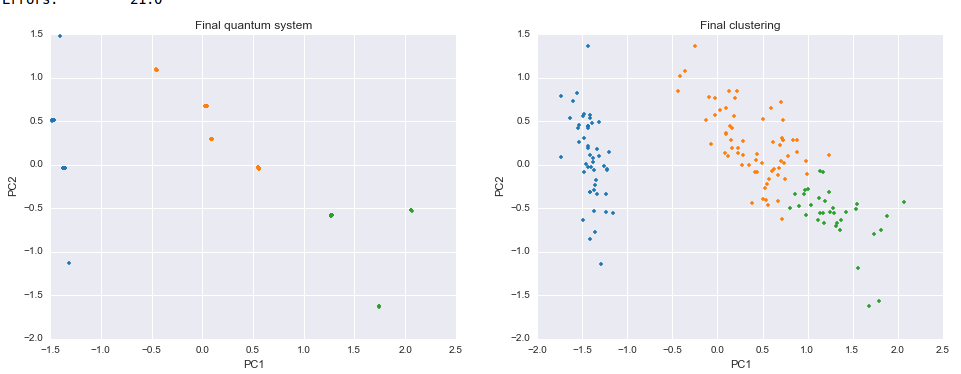
\includegraphics[width=\textwidth]{Horn/img/iris_2pc_cluster.png}
\caption{Plots of the converged data data points and final clustering for 2 PC.}
\label{fig:iris_2pc_cluster}

\end{figure}

For the sake of completeness, Fig. \ref{fig:iris_allpc_cluster} shows the clustering over all PCs. This solution has an accuracy of 82.67\% computed with consistency index.


\begin{figure}[hbtp]
\centering
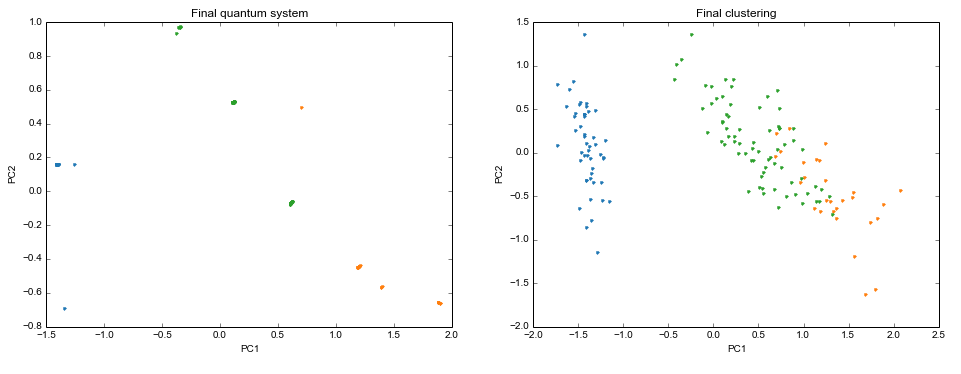
\includegraphics[width=\textwidth]{Horn/img/iris_allpc_cluster.png}
\caption{Plots of the converged data data points and final clustering for all PC of Iris data.}
\label{fig:iris_allpc_cluster}
\end{figure}


\subsubsection{Crab data}


The crabs dataset has 200 samples and describes 5 morphological measurements on 50 crabs each of two colour forms and both sexes (total of 200 crabs), of the species Leptograpsus variegatus collected at Fremantle, Western Australia. After a preprocessing using PCA with covariance matrix and uncentred data, the dataset is represented in Fig. \ref{fig:crab_2pc_covar}.% #TODO add reference to dataset -->

\begin{figure}[hbtp]
\centering
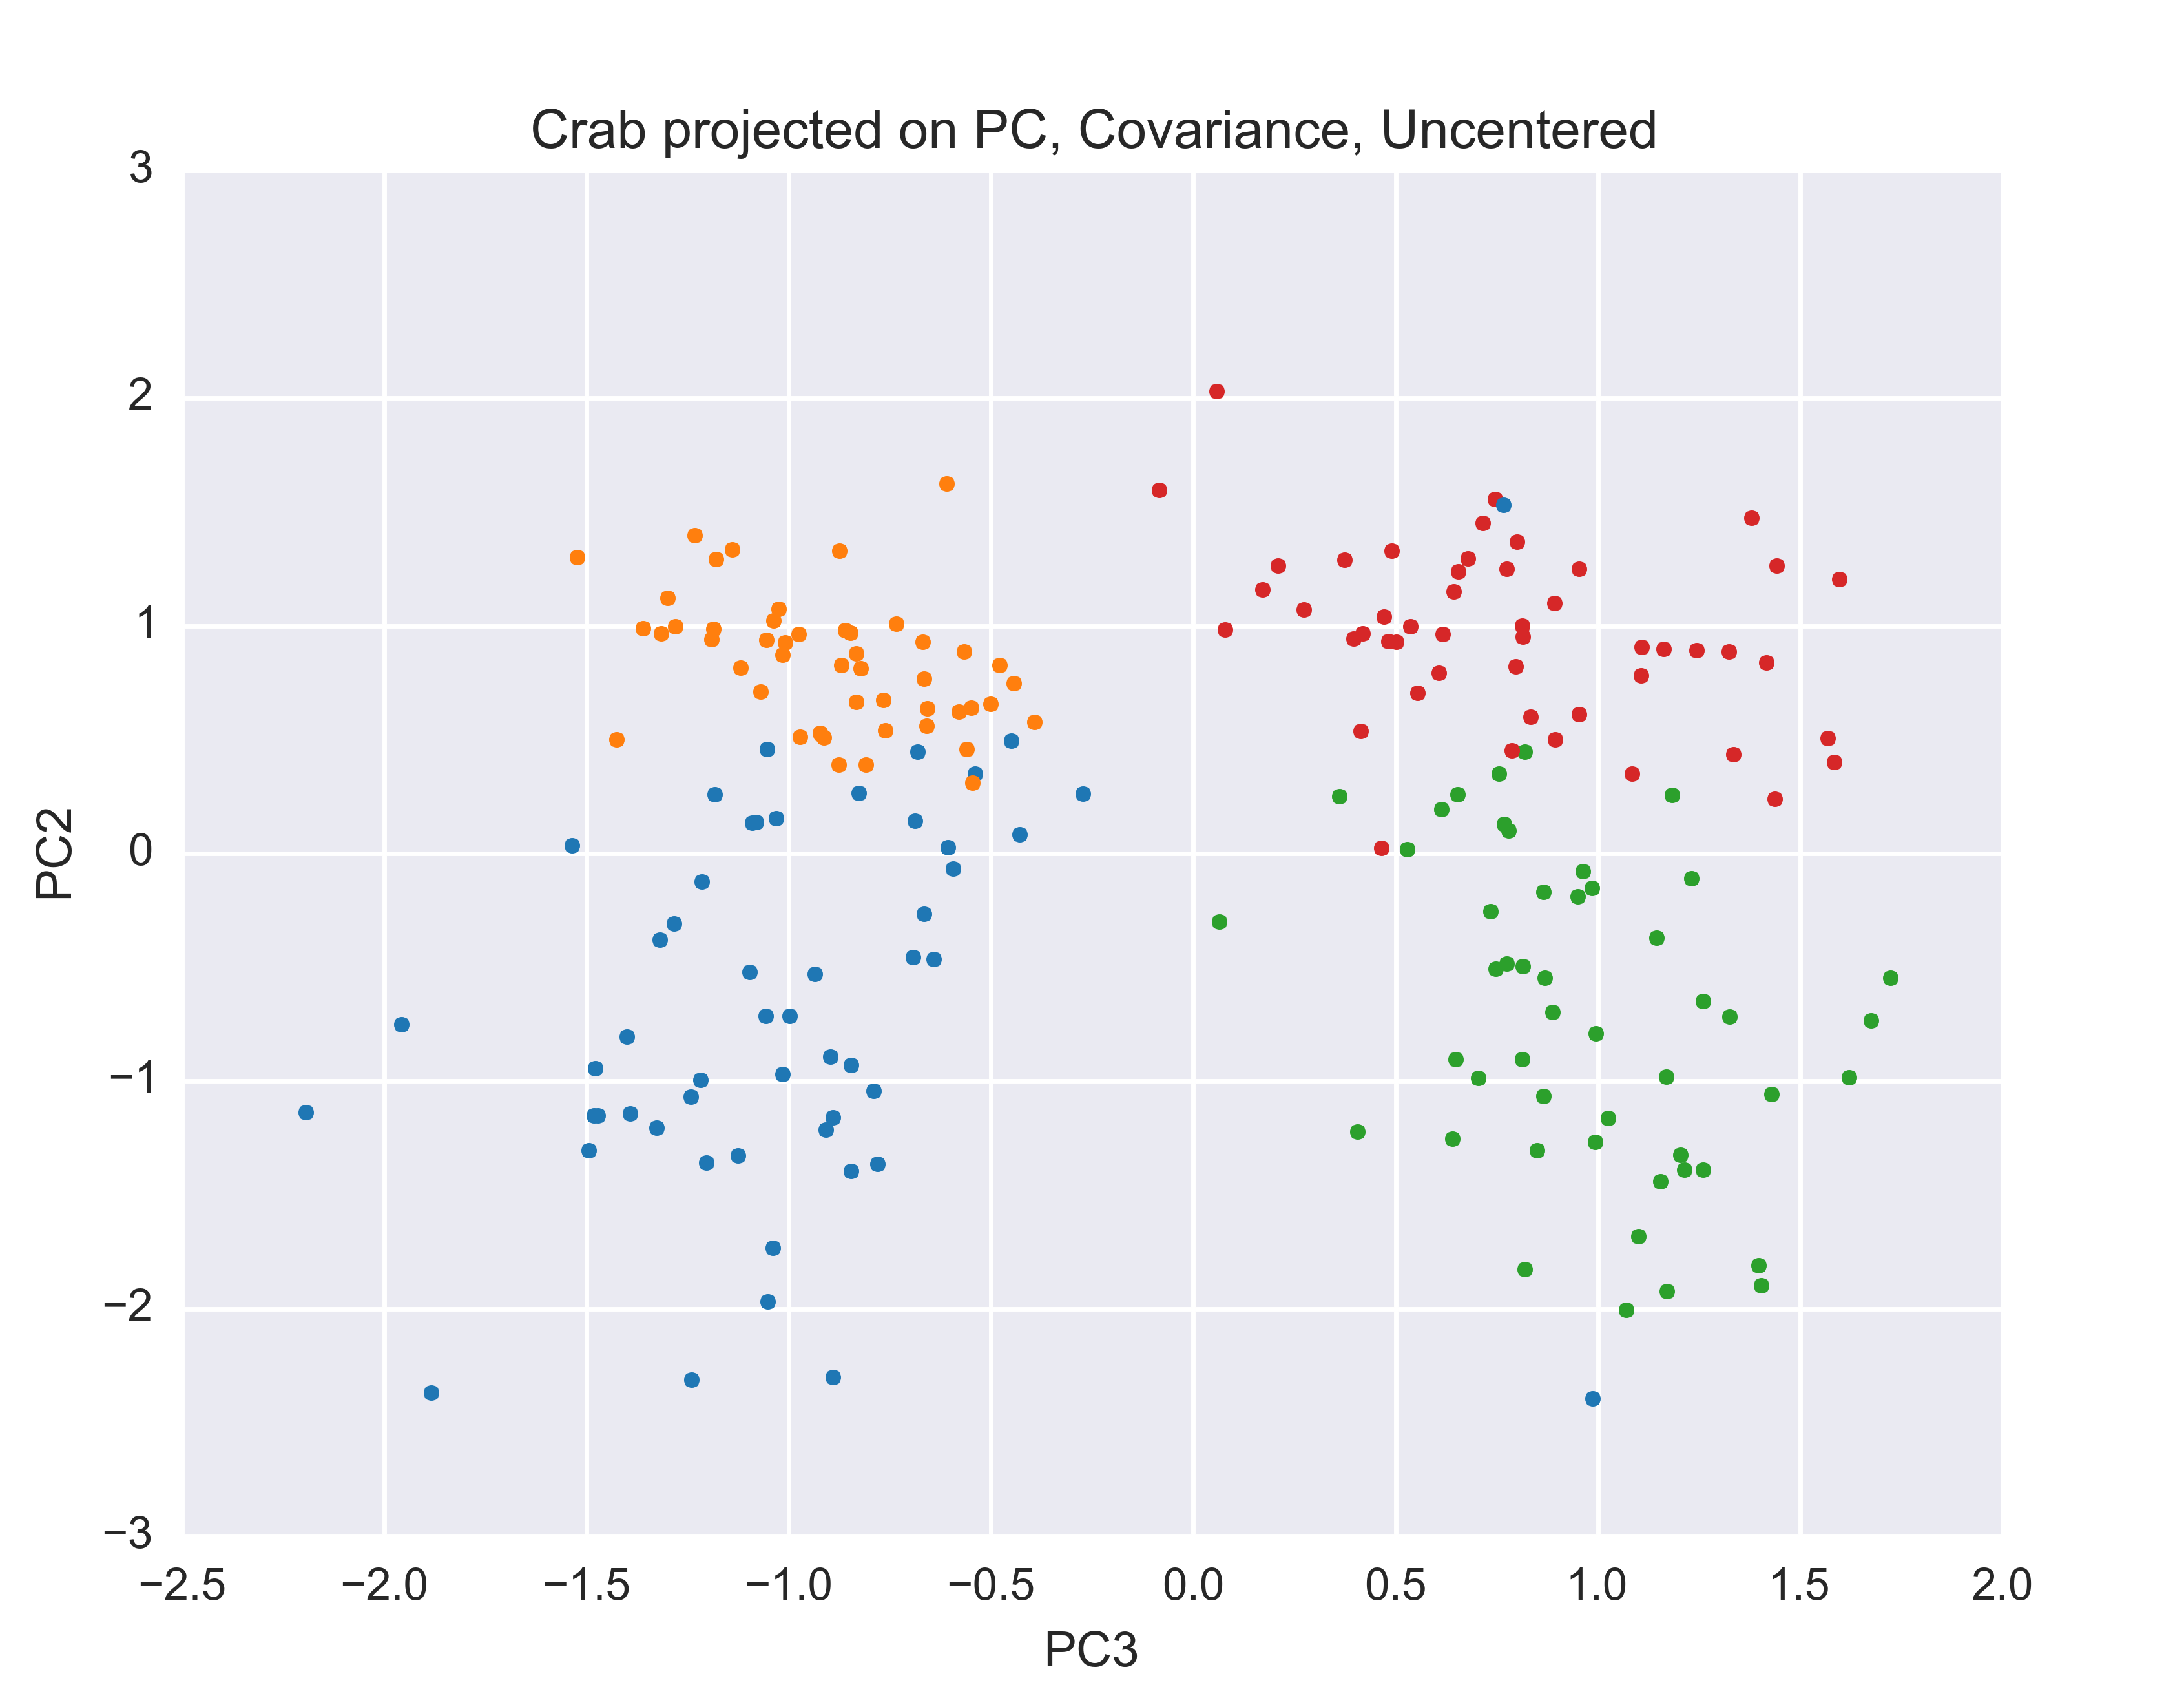
\includegraphics[scale=0.5]{Horn/img/crab_2pc_covar.png}
\caption{Representation of the crab data projected over PC 2 and 3.}
\label{fig:crab_2pc_covar}
\end{figure}

\begin{figure}[hbtp]
\centering
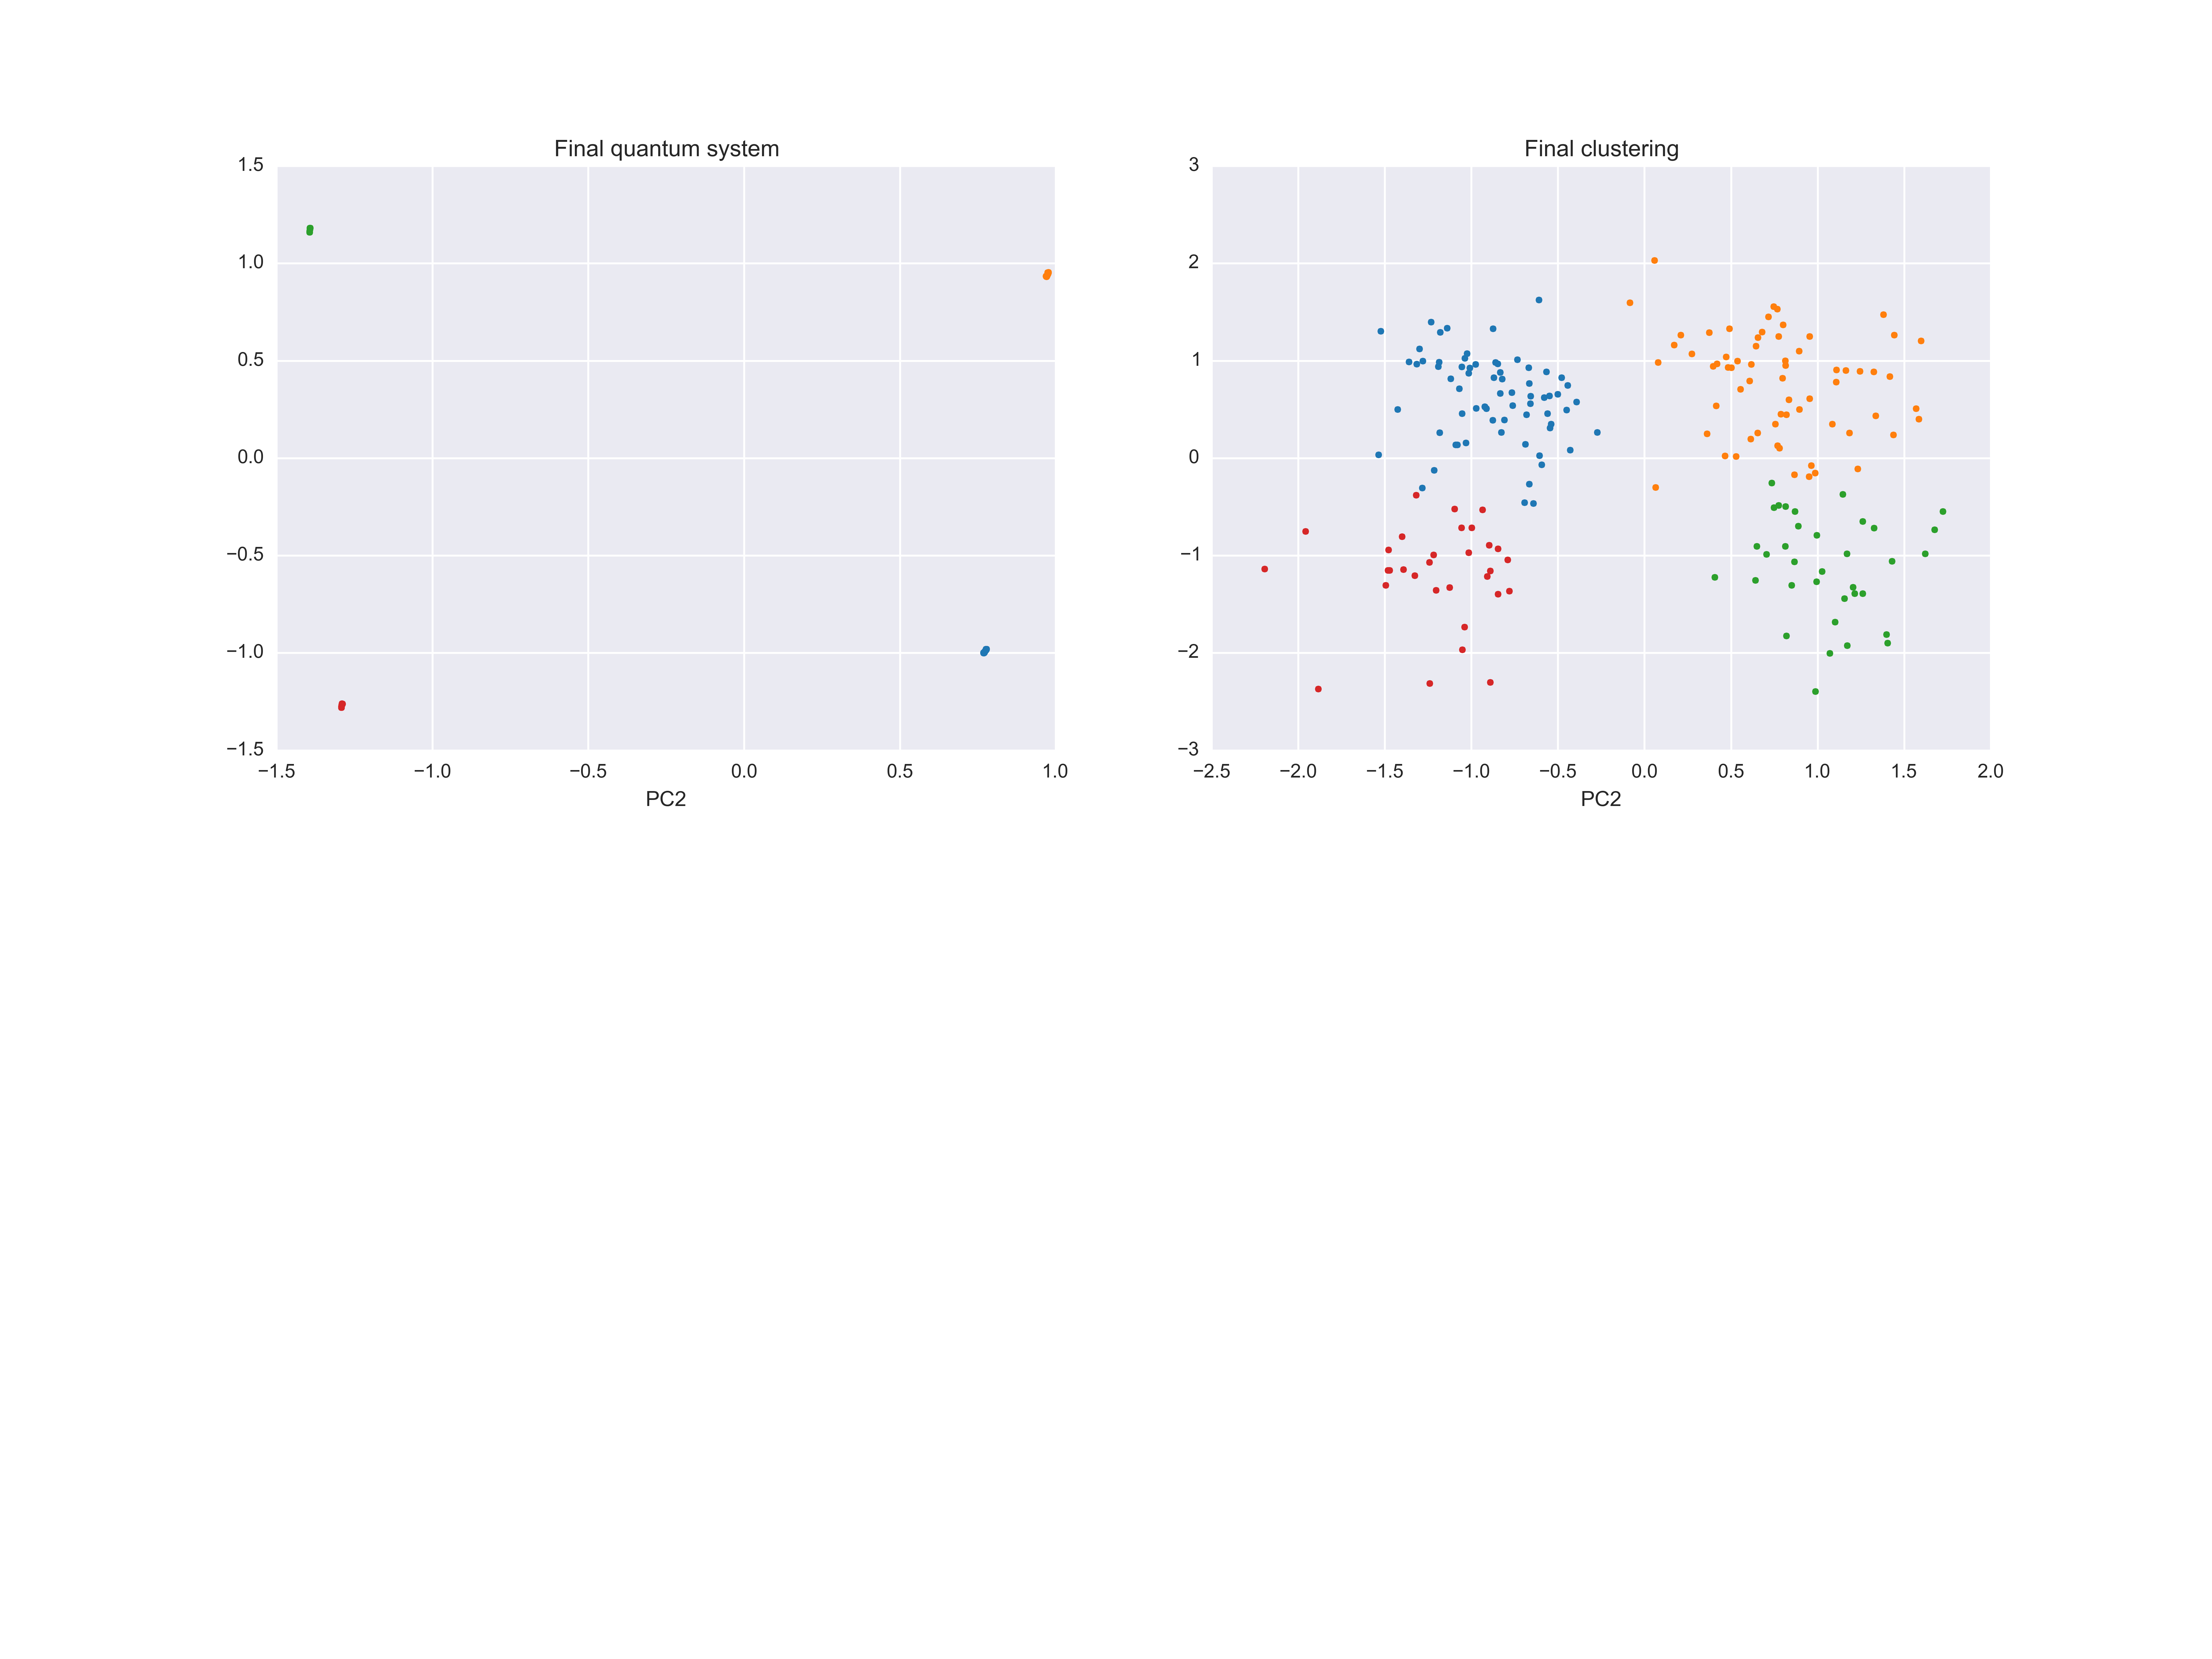
\includegraphics[width=\textwidth]{Horn/img/crab_2pc_covar_cluster.png}
\caption{Representation of the crab data projected over PC 2 and 3.}
\label{fig:crab_2pc_covar_cluster}
\end{figure}

\begin{figure}[hbtp]
\centering
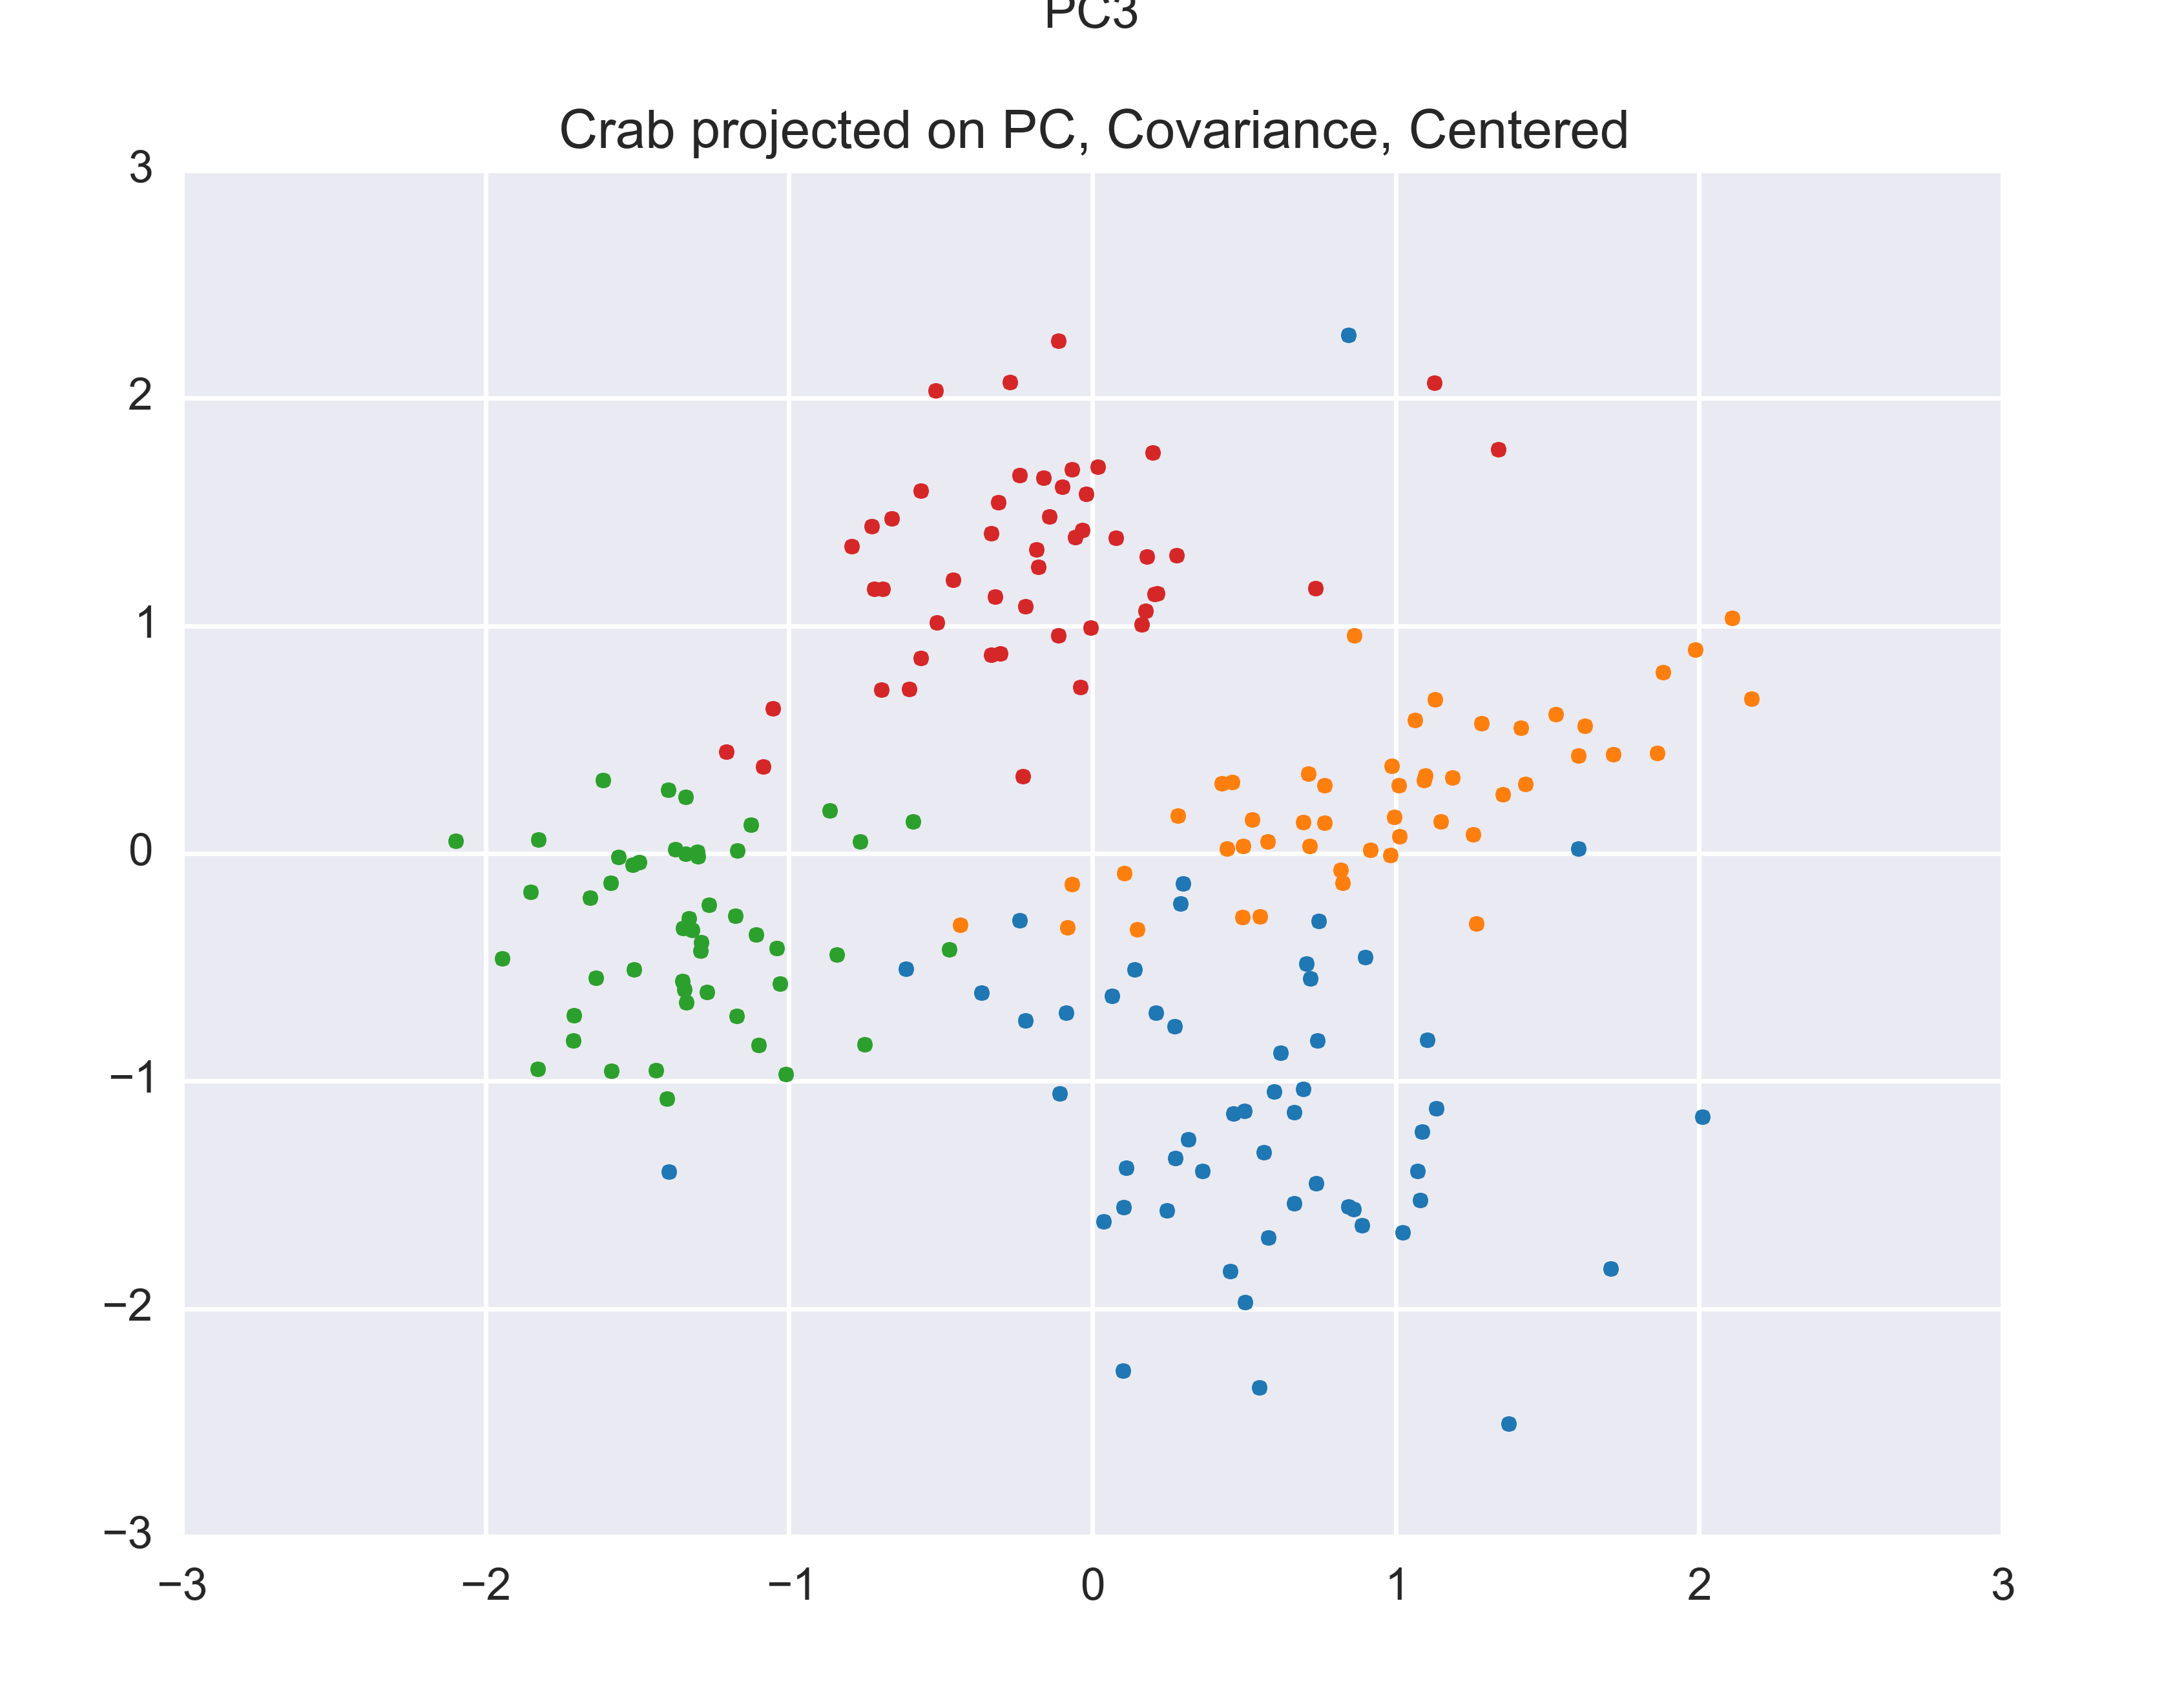
\includegraphics[scale=0.5]{Horn/img/crab_2pc_covar_centered.png}
\caption{Representation of the crab data projected over PC 2 and 3.}
\label{fig:crab_2pc_covar_centered}
\end{figure}

\begin{figure}[hbtp]
\centering
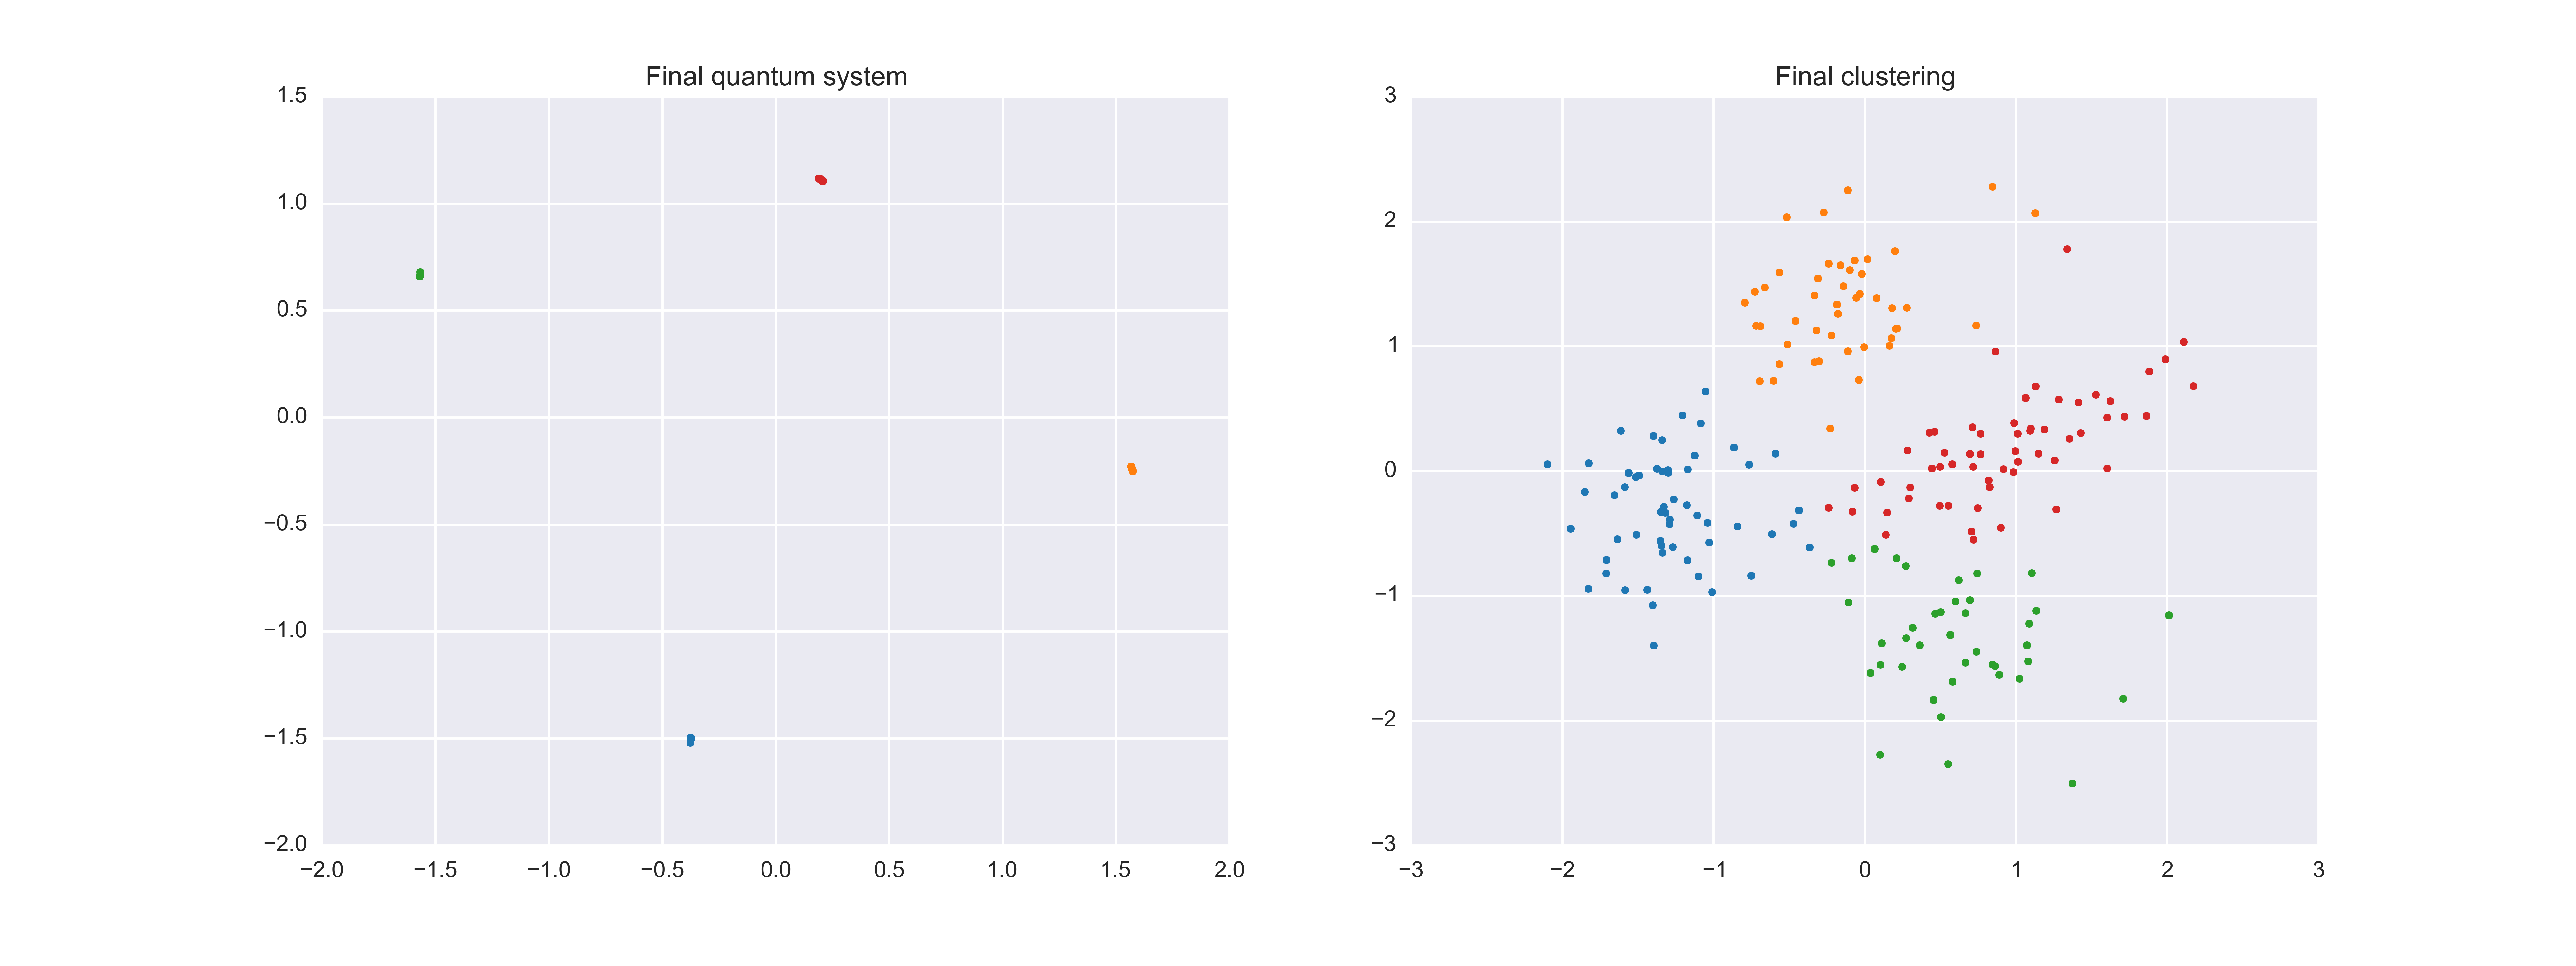
\includegraphics[width=\textwidth]{Horn/img/crab_2pc_covar_centered_cluster.png}
\caption{Representation of the crab data projected over PC 2 and 3.}
\label{fig:crab_2pc_covar_centered_cluster}
\end{figure}


Initial work aimed at reproducing results from [2], but lack of detail on the preprocessing used made it an harder task. Several preprocessings were used, namely whitening or not the data, centring it or not, using covariance versus correlation and different methods of computing the PCs through eigenvalue decomposition or Singular Value Decomposition (SVD). The closest representation to that of the [2] is the one if Fig. C1.


%TODO finish crab

Covariance uncentred consistency index = 0.815
Covariance centred consistency index = 0.91

all pc covariance uncentred consistency index = 0.63
all dimensions original data consistency index = 0.34


\subsection{GPGPU K-Means}




\subsection{K-prototypes influence on coassocs}
%--------------------------------------------%
%--------------------------------------------%
%             CONCLUSIONS
%--------------------------------------------%
%--------------------------------------------%

\section{Conclusion}

% \subsection{Conclusions}
\begin{frame}{Conclusions}
\begin{itemize}
\item Lessons learned: time vs. memory efficiency
\item GPU is a valuable and widely widely available resource for data processing
\item EAC was successfully scaled:
	\begin{itemize}
	\item GPU K-Means
	\item Efficient sparse matrix building
	\item MST equivalence with SL
	\item Disk-based algorithms
	\end{itemize}

\item Contributions:
	\begin{itemize}
	\item Widen the range of EAC's applicability 
	\item New of way of building sparse matrix
	\item New $K_{min}$ rules for sparsity optimizations
	\end{itemize}

\item Plenty of possible extensions

\item Selected parts of this work was compiled and submitted as a conference article

\end{itemize}
\end{frame}

% \subsection{References}
%   \begin{frame}{References}
%       \printbibliography
%   \end{frame}


% blank side for ending
\bgroup
\setbeamercolor{background canvas}{bg=black}
\begin{frame}[plain]{}
\end{frame}
\egroup

\end{document}